% This is samplepaper.tex, a sample chapter demonstrating the
% LLNCS macro package for Springer Computer Science proceedings;
% Version 2.20 of 2017/10/04
%
\documentclass[runningheads]{llncs}
%
\usepackage{graphicx}
% Used for displaying a sample figure. If possible, figure files should
% be included in EPS format.
\usepackage{tikz}
\usetikzlibrary{arrows}
\usepackage{verbatim}
%\usepackage{amsmath}
%\usepackage{amssymb}
%\usepackage{graphicx}
%\usepackage[all]{xy}
\usepackage{array}
\usepackage{enumitem}
%\usepackage{cite}
\usepackage{natbib}
% If you use the hyperref package, please uncomment the following line
% to display URLs in blue roman font according to Springer's eBook style:
% \renewcommand\UrlFont{\color{blue}\rmfamily}
\usepackage[breaklinks=true]{hyperref}
\usepackage{breakcites}
\renewcommand\UrlFont{\color{blue}\rmfamily}

\begin{document}
%
\title{Understanding Program State Through Attestation}
%
%\titlerunning{Abbreviated paper title}
% If the paper title is too long for the running head, you can set
% an abbreviated paper title here
%
\author{Yan Shoshitaishvili\inst{1} \and Perry Alexander\inst{2}}
%
\authorrunning{Y. Shoshitaishvili and P. Alexander}
% First names are abbreviated in the running head.
% If there are more than two authors, 'et al.' is used.
%
\institute{Arizona State University \\
  Tempe, AZ \\
  \email{yans@asu.edu}
  \and
  Institute for Information Sciences \\ The
  University of Kansas \\ Lawrence, KS 66045 \\
  \email{palexand@ku.edu}}
%
\maketitle              % typeset the header of the contribution
%
\begin{abstract}
Runtime remove attestation is understanding program state under constrained
disclosure. A relying party observes and appraises the behavior of a
remote target by executing an attestation protocol. The protocol and the remote
target constrain what can be observed by the relying party.  Designing
attestation protocols requires identifying measurement points in program state
that provide meaningful approximations  while respecting constrained disclosure.
Finding such observation points is complicated by state complexity, difficulty
mapping execution state to behavior, and unavailability of source code.  Static
and dynamic analysis techniques including fuzzing, abstract
interpretation, and decompilation prove effective in approximating system state
for testing and debugging.  We propose repurposing such techniques to discover
measurements of user-space programs that soundly approximate runtime behavior.

\keywords{remote attestation \and static analysis \and runtime measurement \and program understanding.}
\end{abstract}
%
%
%

%%\section{Introduction}

Establishing trust in a remote peer is a challenging problem that requires
approximating program behavior. \citet{Martin:08:The-ten-page-in} defines trust
as exhibiting unambiguous identification, unhindered operation, and direct
observation of good behavior or indirect observation by a trusted third party.
One technique for establishing trust in a target system's execution is semantic
remote attestation~\citep{Haldar:04:Semantic-Remote,Coker::Principles-of-R}.
Shown in Figure~\ref{fig:remote-attestation} a \emph{relying party} ($RP$) sends
an attestation request ($r:(R,n,a)$) to a \emph{target} ($T$) where attestation
generates and returns evidence and meta-evidence ($e:(E,n)$) that can then be \emph{appraised} to determine trust.

\begin{figure}[hbtp]
  \centering
  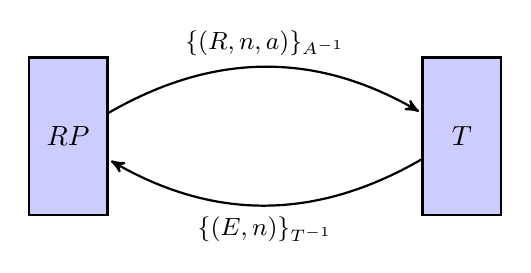
\begin{tikzpicture}[->,>=stealth',shorten >=1pt,auto,node distance=2.0cm,
    thick,main node/.style={rectangle,fill=blue!20,draw,
      font=\sffamily,minimum height=20mm,minimum width=10mm},
    io node/.style={rectangle,
      font=\sffamily,minimum height=5mm,minimum width=10mm}]
    
    \node[main node] (NM) {$RP$};
    \node[main node] (NME) [node distance=5.0cm, right of=NM] {$T$};
%%    \node[io node] (IN) [above of=NM] {$R$};
%%    \node[io node] (OUT) [below of=NM] {$\mathtt{Prop}$};
    
    \path[every node/.style={font=\sffamily\small, fill=white,inner sep=1pt}]
    (NM) edge [bend left=30] node[above=1mm] {$\{(R,n,a)\}_{A^{-1}}$} (NME)
    (NME) edge [bend left=30] node[below=1mm] {$\{(E,n)\}_{T^{-1}}$} (NM)
  %  (IN) edge (NM)
  %  (NM) edge (OUT)
    ;
  \end{tikzpicture}
  \caption{Remote attestation architecture
  showing a \emph{relying party} making an attestation request of a
  \emph{target}.}
  \label{fig:remote-attestation}
\end{figure}

\citet{Coker::Principles-of-R,Coker:08:Attestation:-Ev} define a remote
attestation model where a target executes an \emph{attestation protocol} that
gathers evidence and generates meta-evidence of its execution. The protocol
sequences attestation service execution including measurement, signing, and
making attestation requests of other systems.  These protocols are executed by
one or many \emph{attestation manager(s)} associated with the relying party and target.

Working with MITRE, JHUAPL, and NSA, the University of Kansas has developed the
Copland~\citep{Ramsdell:2019aa} attestation protocol language and the MAESTRO
framework~\citep{petz2022innovations,
Petz:2024:Verified-Configuration-and-Deployment-Paper}
for synthesizing remote attestation systems. Copland is a formally specified
language that sequences the execution of attestation services providers (ASPs)
to gather measurement information, cryptographic operations to generate
meta-evidence, and requests to remote attestation managers for evidence. Using
the Copland formal semantics, verified Coq definitions of attestation, and
synthesis of Coq to CakeML~\citep{Kumar:2014:CVI:2535838.2535841} we have a
formally verified, layered attestation capability guaranteeing that all ASPs are
executed in the right order at the right place.
 
If we understand how an application executes, we can design Copland
protocols and ASPs to gather evidence with a verfied MAESTRO environment.  The
key is understanding and gathering evidence of ``good'' This is evidenced by the
LKIM~\citep{Loscocco:07:Linux-kernel-in} contextual measurement system designed
for gathering evidence and appraising Linux.  LKIM takes advantage of a common,
consistent Linux memory layout to sample memory locations associated with
critical data structures.  These samples are assembled as evidence that is
appraised to establish whether the kernel satisfies policy.

MAESTRO's widespread adoption is limited by difficulty understanding how to
observe \emph{arbitrary} programs.  While the operating system is critical, user
space and other privileged programs may also be compromised by an attack or
misconfiguration.  Understanding ``how to look'' at such programs is frequently
infeasible due to lack of source code and program complexity.  For MAESTRO and
other attestation systems to succeed, the process of defining measurements,
measurement targets, and attestation protocols must be automated.

Arizona State University has developed
techniques to fuzz~\citep{trickel2022toss,salls2020exploring,peng2018t}, symbolically execute~\citep{stephens2016driller,shoshitaishvili2016sok}, and statically analyze~\citep{das2022hybrid,vadayath2022arbiter} complex user space programs and their components, including complex subsystems such as the dynamic allocator (``heap'')~\citep{eckert2018heaphopper} and cross-runtime interface bindings~\citep{dinh2021favocado}.
These techniques prove useful for automatically discovering critical data structures useful for attack and defense.

We propose a spectrum of techniques to automatically discover and
implement high-quality measurement for use in downstream attestation.
When source code is available (increasing the efficacy of static analysis by granting it accurate variable type information), we will use static analysis to identify memory regions whose measurements will be particularly informative.
When source (and variable type information) is not available, we will leverage our decompilation techniques to find system variables whose values prove useful for appraisal, and leverage fuzzing to identify unusual states.
Finally, we propose generating ASPs and instrumenting code during compilation (when source is available) or retrofitting it into the already-compiled binary using our binary modification techniques~\citep{wang2017ramblr} (when source is not available) to provide measurement access to critical structures.

We will use Fuzzing to generate and identify ``weird'' memory states.
Once such states are identified, by analyzing the constraints that must be satisfied to trigger them, we will develop measurement and appraisal routines to detect these memory states.
Because we understand how fuzzing is performed, and can leverage symbolic execution to delve deeper into the functionality of the program, we can understand what measurements tell us about observed memory.

Program decompilation identifies critical system variables for runtime measurement.
Decompilation produces source with variables present.
Once decompiled, we will perform source-level analysis to determine what variables are valuable for runtime measurement.
Using type information, we can bound memory values and identify good and bad variable values.
Using this information, we can automatically synthesize measurement and appraisal routines for variable memory locations.

We plan to use static analysis and compilation techniques to automatically generate measurement and appraisal routines from OS and user-space software.
For example, we can utilize our dynamic allocator analysis results~\citep{eckert2018heaphopper} to synthesize measurement routines for allocator implementation to detect integrity violations due to other bugs in the program.
We can carry out similar intervention at the boundary between different program components by leveraging interface specifications combined with advanced analysis~\citep{dinh2021favocado}.

We must take care to limit the performance impact of measurement instrumentation.
In other words, the measurement should be triggered as rarely as possible during runtime while still providing detection guarantees.
This problem is an interesting mirror to false positive reduction during static analysis.
By leveraging our system of \emph{Iterative False Positive Reduction} using a combination of Abstract Interpretation and Dynamic Symbolic Execution~\citep{vadayath2022arbiter}, we can narrow down to increasingly reduced instrumentation sites (by disproving the need for instrumentation at given points in the program), reducing runtime overhead by trading it for analysis-time cost.
Even in cases where we cannot disprove the need for instrumentation, we may be able to ``back-propagate'' certain constraints that, if satisfied, disprove the need for further measurement at runtime.
By carefully crafting such runtime instrumentation and correlating it to marked memory locations and events, we can essentially synthesize ``tripwires' that, when not tripped, cause very little overhead.


% 
% 
% ---- Bibliography ----
%
% BibTeX users should specify bibliography style 'splncs04'.
% References will then be sorted and formatted in the correct style.
%
%\bibliographystyle{splncs04}
\bibliographystyle{splncsnat}
\bibliography{bib/sldg}
%
\end{document}
